%\subsection{Google Cloud Messaging}

	\par No momento em que é lançada alguma nota, falta ou prova agendada, o
\textit{web service} precisa transmitir esta informação para o aplicativo
Android. Para que esta comunicação aconteça foi utilizado o serviço da Google
chamado de Google Cloud Messaging (GCM).

	\par Neste contexto, o servidor \textit{web} envia uma mensagem para o GCM com
as informações que precisa passar para a aplicação \textit{mobile}. A partir
daí, a entrega dos dados para os dispositivos móveis fica por conta da Google.

	\par Para que o GCM apresentasse o resultado esperado, foi preciso acessar o
site Google \textit{Developers Console} através do endereço
\url{https://console.developers.google.com} e construir um novo projeto. Para
criá-lo, bastou clicar no botão \textit{Create Project} que está na página
inicial, conforme pode se ver na Figura \ref{fig:gcm}. Logo após, foi
adicionado um nome ao projeto e clicado no botão criar, como mostra a Figura
\ref{fig:gcm1}.

	
	%figura 1
	\begin{figure}[h!] 
		\centerline{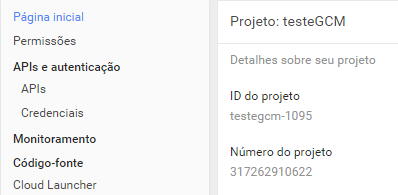
\includegraphics[scale=0.6]{./imagens/2_q_metodologico/4_procedimentos_resultados/41_gcm/gcm.png}}
		\caption[Criando um novo projeto]{Criando um novo projeto.
		\textbf{Fonte:}Elaborado pelos autores.}
		\label{fig:gcm}
	\end{figure}
	
	\begin{figure}[h!] 
		\centerline{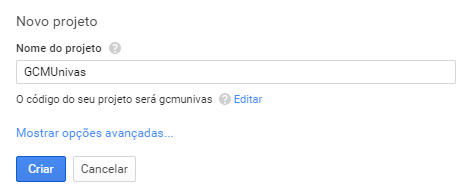
\includegraphics[scale=0.7]{./imagens/2_q_metodologico/4_procedimentos_resultados/41_gcm/gcm1.png}}
		\caption[Inserindo o nome do projeto]{Inserindo o nome do projeto.
		\textbf{Fonte:}Elaborado pelos autores.}
		\label{fig:gcm1}
	\end{figure}
	
	\pagebreak
	
	\par Ao criar o projeto foi aberta uma tela para sua configuração, ilustrada na
Figura \ref{fig:gcm2}.

	\begin{figure}[h!] 
		\centerline{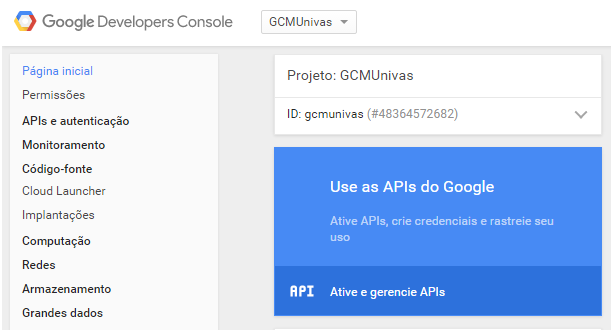
\includegraphics[scale=0.7]{./imagens/2_q_metodologico/4_procedimentos_resultados/41_gcm/gcm2.png}}
		\caption[Tela de configuração do projeto]{Tela de configuração do projeto.
		\textbf{Fonte:}Elaborado pelos autores.}
		\label{fig:gcm2}
	\end{figure}
		
	\par O primeiro dado que se obteve foi o número do projeto, também chamado de
\textit{Sender} ID. Este código serve para que a Google reconheça a aplicação
que enviou a mensagem. Para visualizar este identificador, foi preciso clicar
nos detalhes do projeto na página inicial, como se vê na Figura \ref{fig:gcm3}.

	\begin{figure}[h!] 
		\centerline{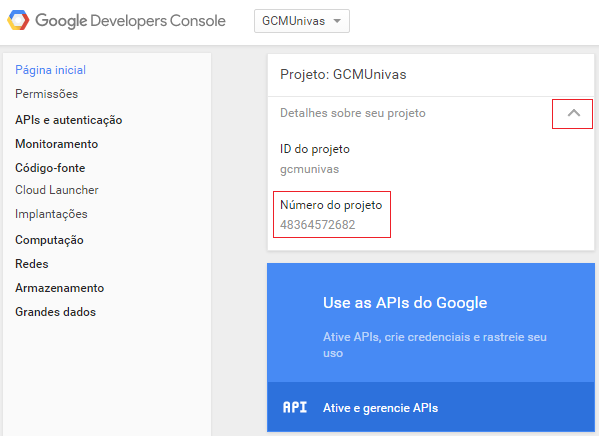
\includegraphics[scale=0.65]{./imagens/2_q_metodologico/4_procedimentos_resultados/41_gcm/gcm3.png}}
		\caption[Número do projeto]{Número do projeto.
		\textbf{Fonte:}Elaborado pelos autores.}
		\label{fig:gcm3}
	\end{figure}
	
	\par O próximo passo, foi habilitar a API GCM para trabalhar com o projeto.
Para essa etapa, foi necessário ir na aba APIs e autenticação, selecionando a
opção APIs, conforme indica a Figura \ref{fig:gcm4}. Na tela presente aparecem
os serviços fornecidos pela Google. Neste caso optou-se por \textit{Cloud
Messaging for Android}, também ilustrado na Figura \ref{fig:gcm4}.

	\begin{figure}[h!] 
		\centerline{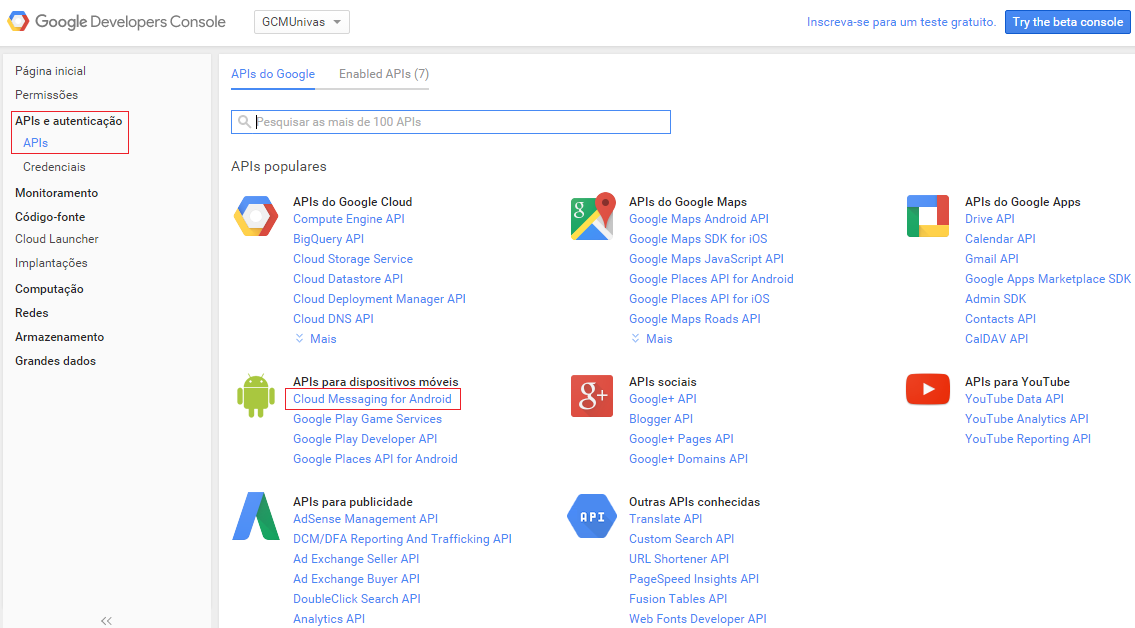
\includegraphics[scale=0.4]{./imagens/2_q_metodologico/4_procedimentos_resultados/41_gcm/gcm4.png}}
		\caption[Habilitando GCM para Android]{Habilitando GCM para Android.
		\textbf{Fonte:}Elaborado pelos autores.}
		\label{fig:gcm4}
	\end{figure}
	
	\par Ao selecionar \textit{Cloud Messaging for Android}, foi apesentada a
tela com a opção de ativar o GCM ao projeto, como mostra a Figura \ref{fig:gcm5}.

	\begin{figure}[h!] 
		\centerline{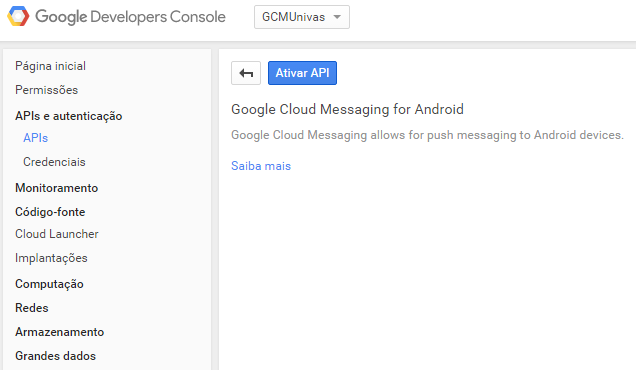
\includegraphics[scale=0.66]{./imagens/2_q_metodologico/4_procedimentos_resultados/41_gcm/gcm5.png}}
		\caption[Botão para ativar o GCM ao projeto]{Botão para ativar o GCM ao projeto.
		\textbf{Fonte:}Elaborado pelos autores.}
		\label{fig:gcm5}
	\end{figure}
	
	\pagebreak

	\par Para concluir a configuração, foi preciso acessar a aba APIs e
autenticação novamente, escolhendo a alternativa Credenciais, como mostra a
Figura \ref{fig:gcm6}. Na página apresentada, foi selecionada a opção Chave de
API, igualmente exibido na Figura \ref{fig:gcm6}.

	\begin{figure}[h!] 
		\centerline{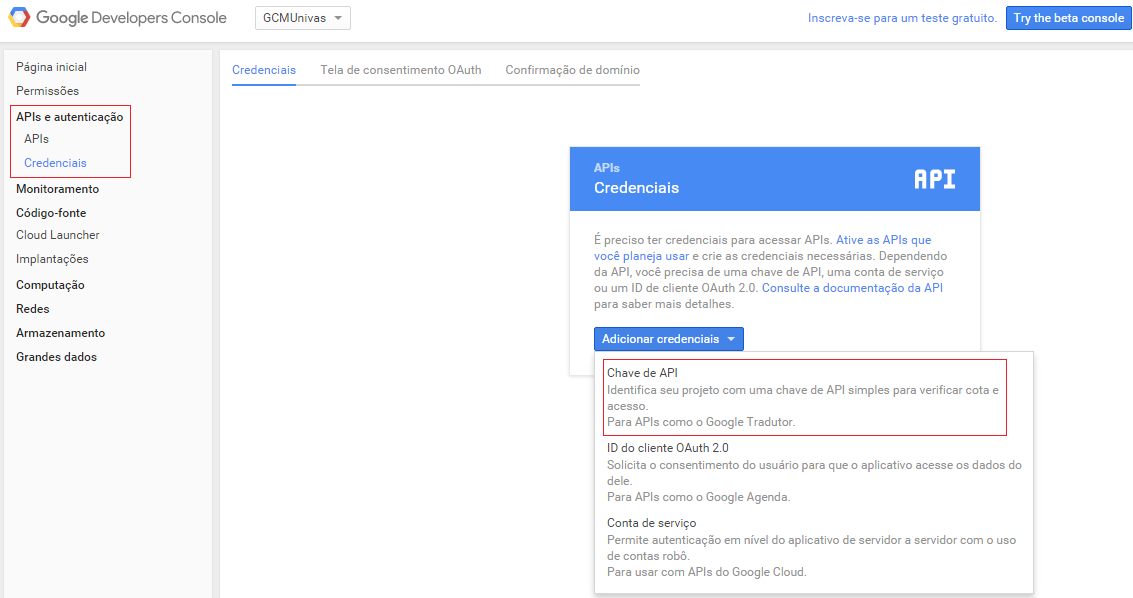
\includegraphics[scale=0.4]{./imagens/2_q_metodologico/4_procedimentos_resultados/41_gcm/gcm6.png}}
		\caption[Criando as credenciais]{Criando as credenciais.
		\textbf{Fonte:}Elaborado pelos autores.}
		\label{fig:gcm6}
	\end{figure}
	
	\par Ao escolher Chave de API, foi exibida uma tela a qual se escolheu a opção
Chave de Servidor, demostrado na Figura \ref{fig:gcm7}.

	\begin{figure}[h!] 
		\centerline{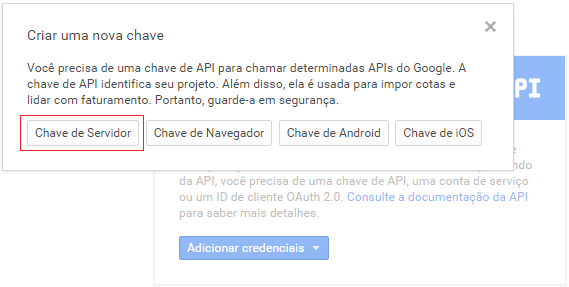
\includegraphics[scale=0.7]{./imagens/2_q_metodologico/4_procedimentos_resultados/41_gcm/gcm7.png}}
		\caption[Escolhendo a opção Chave de Servidor]{Escolhendo a opção Chave de Servidor.
		\textbf{Fonte:}Elaborado pelos autores.}
		\label{fig:gcm7}
	\end{figure}

	\par Ao decidir-se por Chave de Servidor, foi apresentada uma tela onde é
criada a chave pública, também conhecida por \textit{Sender Auth Token}. Esta
identificação é transmitida no cabeçalho das mensagens enviadas do servidor ao
GCM. Para que esse código fosse gerado foi fundamental adicionar um nome e o IP
do \textit{web service}, como mostra a Figura \ref{fig:gcm8}. Ao clicar no
botão criar, a Google apresentou a chave gerada, como ilustra a Figura
\ref{fig:gcm9}.

	\begin{figure}[h!] 
		\centerline{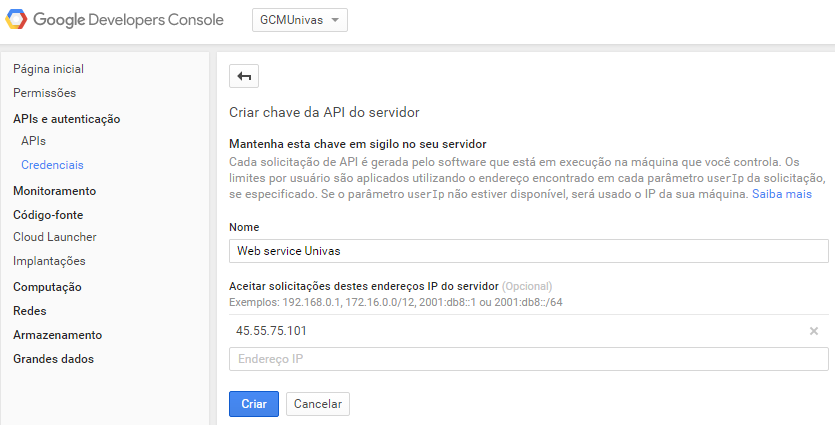
\includegraphics[scale=0.55]{./imagens/2_q_metodologico/4_procedimentos_resultados/41_gcm/gcm8.png}}
		\caption[Inserindo dados do servidor]{Inserindo dados do servidor.
		\textbf{Fonte:}Elaborado pelos autores.}
		\label{fig:gcm8}
	\end{figure}
	
	\begin{figure}[h!] 
		\centerline{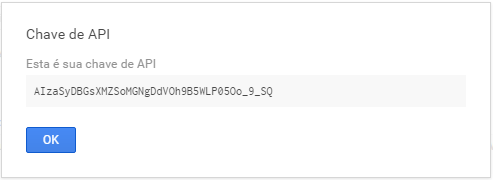
\includegraphics[scale=0.7]{./imagens/2_q_metodologico/4_procedimentos_resultados/41_gcm/gcm9.png}}
		\caption[Chave de API gerada]{Chave de API gerada.
		\textbf{Fonte:}Elaborado pelos autores.}
		\label{fig:gcm9}
	\end{figure}
